%% Ankur Sinha

%% packages %%
% support for coloured text
\usepackage{color}
% IPA
\usepackage{tipa}
\usepackage[scale=2]{ccicons}
\usepackage{amssymb}
% Define the colours we use for E and I in all graphs
\usepackage{jneurosci}
\usepackage{subcaption}
\usepackage[T1]{fontenc}
\usepackage[utf8]{inputenc}
% \usepackage[style=nature,backend=biber,autocite=footnote]{biblatex}
% \addbibresource{/home/asinha/Documents/01_Readables/00_research_papers/bibliography/masterbib.bib}
% \renewcommand*{\bibfont}{\tiny}
% Use opensans
% \usepackage[default,scale=0.95]{opensans}
\usepackage[sfdefault]{roboto}
% for strike through
\usepackage[normalem]{ulem}
% links, urls, refs
\definecolor{links}{HTML}{2A1B81}
% Fedora blue for the theme
\definecolor{FedoraBlue}{HTML}{2A1B81}
\usepackage{hyperref}
\hypersetup{colorlinks,linkcolor=Green,urlcolor=links}
% graphics
\usepackage{graphicx}
% algorithm
\usepackage{algorithmic}
\usepackage{textcomp}
\usepackage{wrapfig}
\usepackage{textgreek}
\usepackage{euler}
\usepackage{tabularx}
\usepackage{booktabs}
\usepackage{minted}
\usepackage{csquotes}
% beamer theme
% use defaults for theme
\usetheme[numbering=fraction]{metropolis}
\usefonttheme[onlymath]{serif}
\setbeamerfont{footnote}{size=\tiny}
\setbeamerfont{caption}{size=\tiny}
\setbeamercolor{alerted text}{fg=Green}
\setbeamerfont{note page}{size=\small}

% Not needed in metropolis, but in general footnote citation fixes: https://tex.stackexchange.com/questions/44217/how-can-i-stop-footcite-from-hijacking-my-beamer-columns
% how to use multiple references to the same footnote: https://tex.stackexchange.com/questions/27763/beamer-multiple-references-to-the-same-footnote

% Disable footnoterule
\renewcommand{\footnoterule}{}

%% title %%
\title{NeuroML update}
\author[Ankur Sinha]{Ankur Sinha}
\date{21/09/2022}

%% document begins %%
\begin{document}


% title frame %%
\begin{frame}
  \titlepage{}
\end{frame}
%% Three slides for 5 minutes seems good
%% So, 30 slides at most for 50 minutes
\begin{frame}[c]
  \frametitle{What we've been up to on the NeuroML front}
  \begin{itemize}
    \item Google summer of code (GSoC)
    \item Paper and general improvements
  \end{itemize}
\end{frame}
\section{Google Summer of Code}
\begin{frame}[c]
  \frametitle{GSoC}
  \begin{itemize}
    \item Under the INCF organisation
      \begin{itemize}
        \item 40 accepted this year, in total
        \item No longer limited to students
      \end{itemize}
      \pause{}
    \item Us: 4 candidates
      \begin{itemize}
        \item 3 working on NeuroML/modelling
        \item 1 on NWB
        \item 175 hours each, over 3 months (medium projects)
      \end{itemize}
      \pause{}
    \item Goals:
      \begin{itemize}
        \item Conversions of models to NeuroML (to allow them to be re-used and featured on OSB)
        \item Get folks looking into and using NeuroML in different use cases
          \pause{}
        \item Get folks to improve NeuroML where possible
      \end{itemize}
  \end{itemize}
\end{frame}
\begin{frame}[c]
  \frametitle{GSoC:\ Anuja:\ convert Allen Institute models to NeuroML}
  \begin{itemize}
    \item Masters student at the Bernstein Centre for Computational Neuroscience, Berlin.
      \pause{}
    \item Source models: \href{http://celltypes.brain-map.org/}{Allen institutes cell type database} (\href{http://celltypes.brain-map.org/experiment/electrophysiology/474626527}{example})
      \pause{}
    \item Steps:
      \begin{itemize}
        \item Automate download of models using the Allen SDK
        \item Automate conversion to NeuroML
        \item Plot comparison graphs to validate conversions (\href{https://github.com/OpenSourceBrain/AllenInstituteNeuroML/tree/master/CellTypesDatabase/models/GLIF}{LIF models}, \href{https://github.com/OpenSourceBrain/AllenInstituteNeuroML/tree/master/CellTypesDatabase/models}{Detailed})
        \item Document comparison, usage, update OMV tests for CI
      \end{itemize}
  \end{itemize}
\end{frame}
\begin{frame}[c]
  \frametitle{GSoC:\ Anuja:\ example figure I}
  \begin{figure}[h]
    \centering
    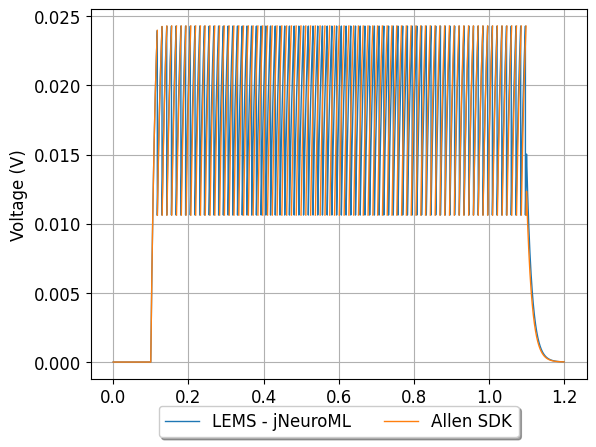
\includegraphics[width=0.9\textwidth]{99_images/Comparison_129pA}
    \caption{Membrane potentials of Allen and NeuroML models}%
    \label{fig:99_images-Comparison_129pA}
  \end{figure}
\end{frame}
\begin{frame}[c]
  \frametitle{GSoC:\ Anuja:\ example figure II}
  \begin{figure}[h]
    \centering
    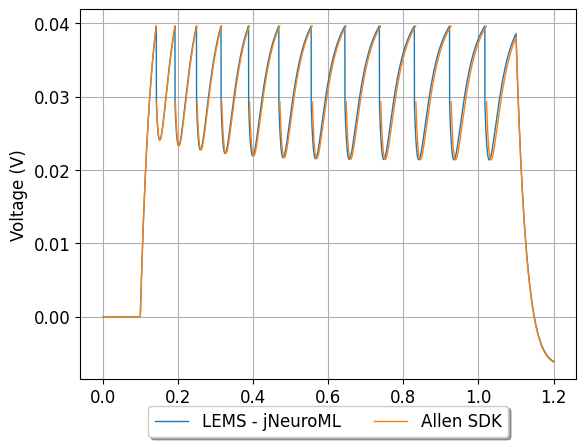
\includegraphics[width=0.9\textwidth]{99_images/Comparison_170pA}
    \caption{Membrane potentials of Allen and NeuroML models}%
    \label{fig:99_images-Comparison_170pA}
  \end{figure}
\end{frame}
\begin{frame}[c]
  \frametitle{GSoC:\ Anuja:\ example figure III}
  \begin{figure}[h]
    \centering
    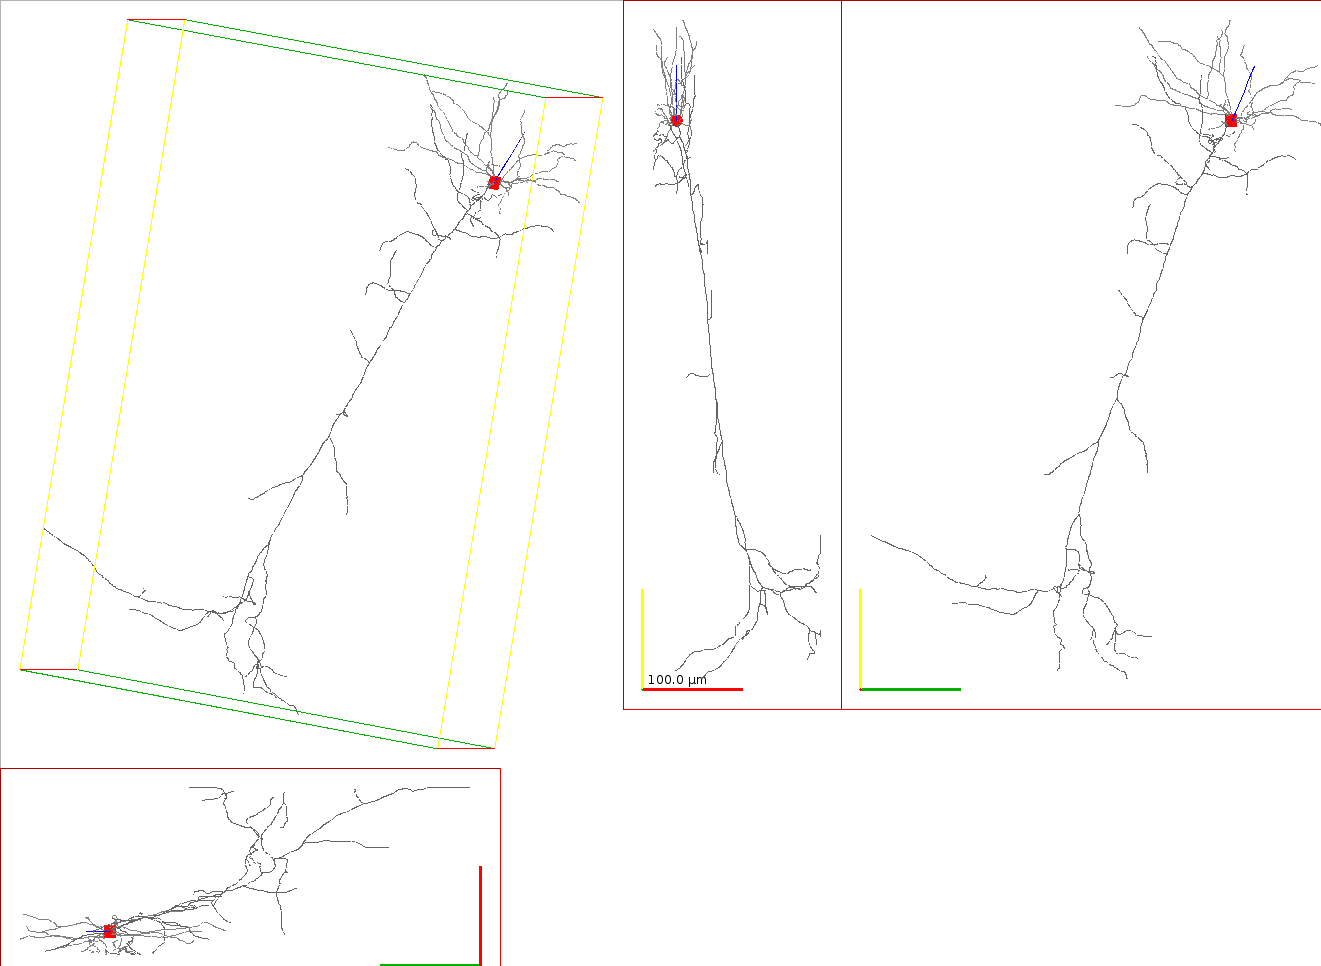
\includegraphics[width=0.9\textwidth]{99_images/Cell_497232312.cell}
    \caption{Morphology of example cell}%
    \label{fig:99_images-morph}
  \end{figure}
\end{frame}
\begin{frame}[c]
  \frametitle{GSoC:\ Anuja:\ example figure IV}
  \begin{figure}[h]
    \centering
    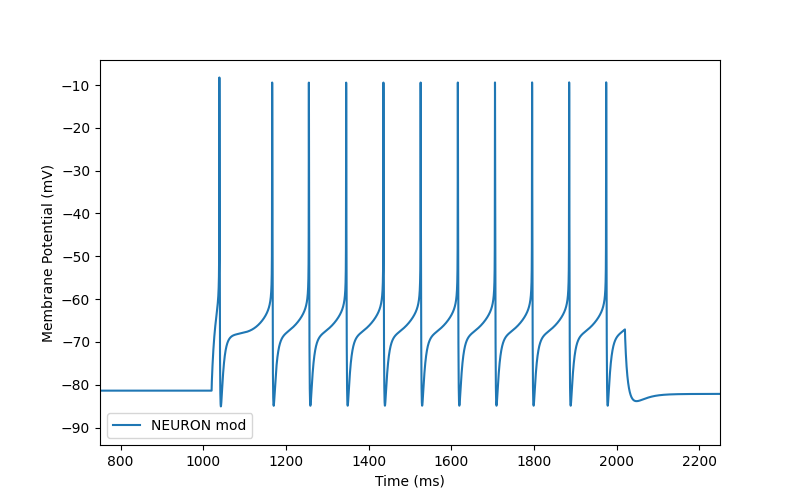
\includegraphics[width=0.55\textwidth]{99_images/NEURON_497232312}\\
    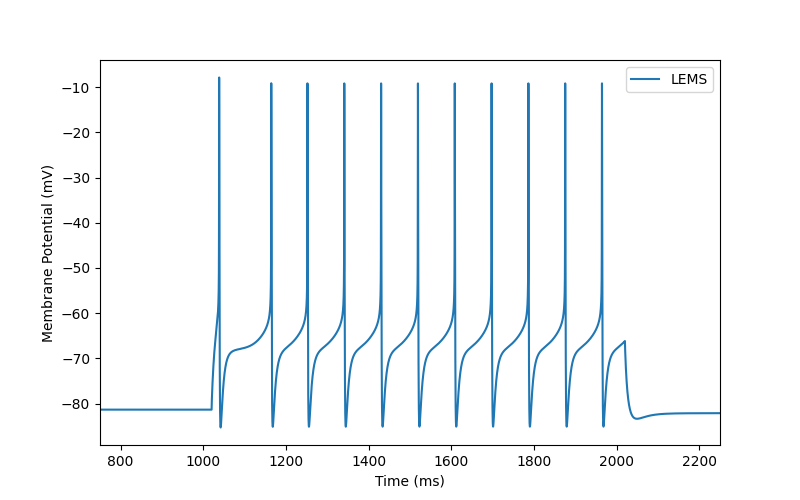
\includegraphics[width=0.55\textwidth]{99_images/LEMS_497232312}
    \caption{NEURON vs NeuroML output}%
    \label{fig:99_images-anuja-neuron-neuroml}
  \end{figure}
\end{frame}
\begin{frame}[c]
  \frametitle{GSoC:\ Shayan:\ convert BahlEtAl2012 (Reduced L5 Pyr Cell) to NeuroML}
  \begin{itemize}
    \item MSc/BSc from IIT Kharagpur (Maths and Computing)
      \pause{}
    \item Source models: \href{https://github.com/OpenSourceBrain/BahlEtAl2012_ReducedL5PyrCell}{OSB/BahlEtAl2012}
      \pause{}
    \item Steps:
      \begin{itemize}
        \item Convert ion channels to NeuroML, validate, \href{https://github.com/OpenSourceBrain/BahlEtAl2012_ReducedL5PyrCell/tree/master/NeuroML2/compare_nml2_mods}{compare with NEURON mod files}
        \item Implement single compartment cell model with passive channels
          \begin{itemize}
            \item incrementally add ion channels
            \item compare with NEURON model
          \end{itemize}
        \item Implement multi-compartmental cell, repeat
        \item \href{https://github.com/OpenSourceBrain/BahlEtAl2012_ReducedL5PyrCell/tree/master/NeuroML2}{Document comparison, usage}, update OMV tests for CI
        \item \href{https://github.com/OpenSourceBrain/BahlEtAl2012_ReducedL5PyrCell/blob/master/NeuroML2/interactive_nml.ipynb}{Interactive notebook} to reproduce figures from paper using NeuroML models
      \end{itemize}
  \end{itemize}
\end{frame}
\begin{frame}[c]
  \frametitle{GSoC:\ Shayan:\ example figures}
  \begin{figure}[h]
    \centering
    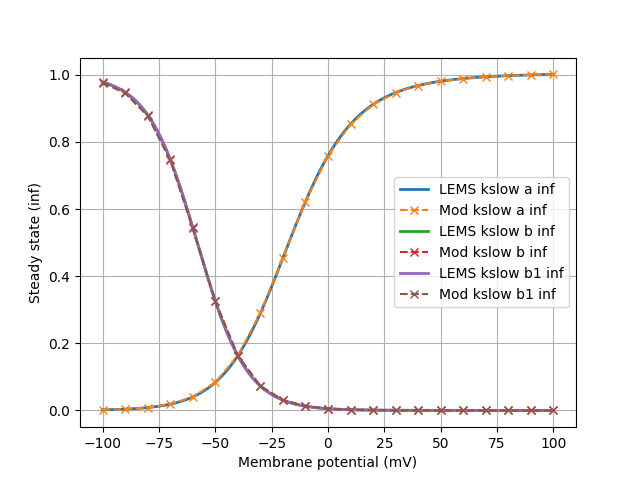
\includegraphics[width=0.48\textwidth]{99_images/kslow.inf}
    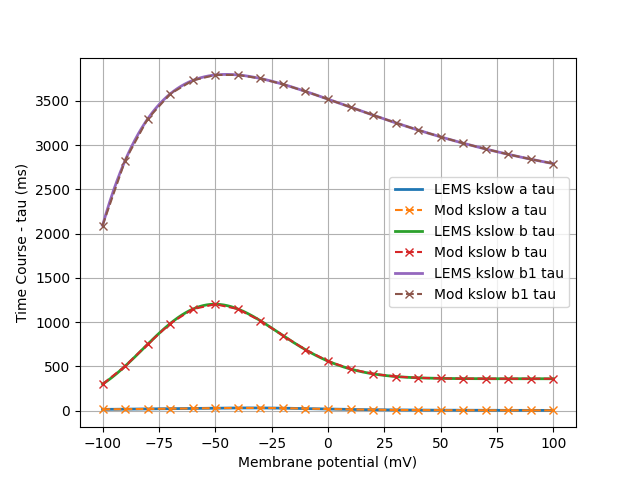
\includegraphics[width=0.48\textwidth]{99_images/kslow.tau}
    \caption{Comparing ion channels: steady state, time constant}%
    \label{fig:99_images-shayan-comparison}
  \end{figure}
\end{frame}
\begin{frame}[c]
  \frametitle{GSoC:\ Shayan:\ example figures II}
  \begin{figure}[h]
    \centering
    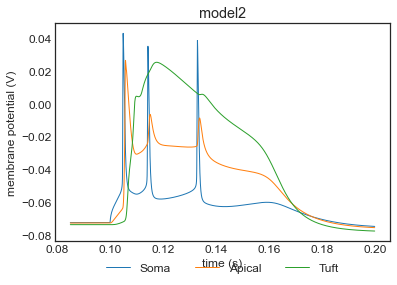
\includegraphics[width=0.55\textwidth]{99_images/output_d}\\
    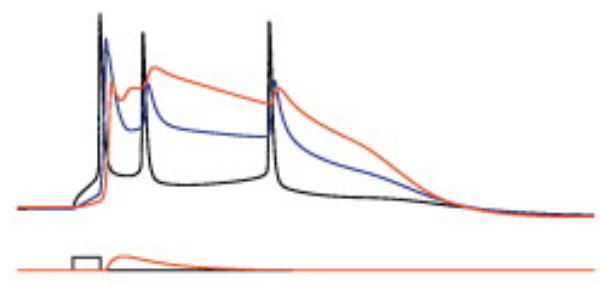
\includegraphics[width=0.52\textwidth]{99_images/shayan-bahl-d}
    \caption{Replicating figures from the paper (8d)}%
    \label{fig:99_images-shayan-comparison-2}
  \end{figure}
\end{frame}
\begin{frame}[c]
  \frametitle{GSoC:\ Rahul:\ convert HH tutorial to Jupyter notebook}
  \begin{itemize}
    \item Aerospace engineer (MTech, IIT Kharagpur), working in South Korea
      \pause{}
    \item Source models: \href{https://github.com/openworm/hodgkin_huxley_tutorial/}{OpenWorm/HH tutorial}
      \pause{}
    \item Steps:
      \begin{itemize}
        \item Investigate Jupyter widgets
        \item Convert pure Python HH tutorial to use Jupyter widgets
        \item Investigate NeuroML based tutorial
        \item Investigate conversion of NeuroML to Jupyter widgets
        \item Update sphinx documentation for \href{https://hodgkin-huxley-tutorial.readthedocs.io/en/latest/}{ReadTheDocs site}
        \item \href{https://github.com/openworm/hodgkin_huxley_tutorial/blob/master/notebooks/GSoC_2022_Submission/GSoC_Documentation.md}{Document usage}.
      \end{itemize}
  \end{itemize}
\end{frame}
\begin{frame}[c]
  \frametitle{GSoC:\ Rahul:\ example I}
  \begin{figure}[h]
    \centering
    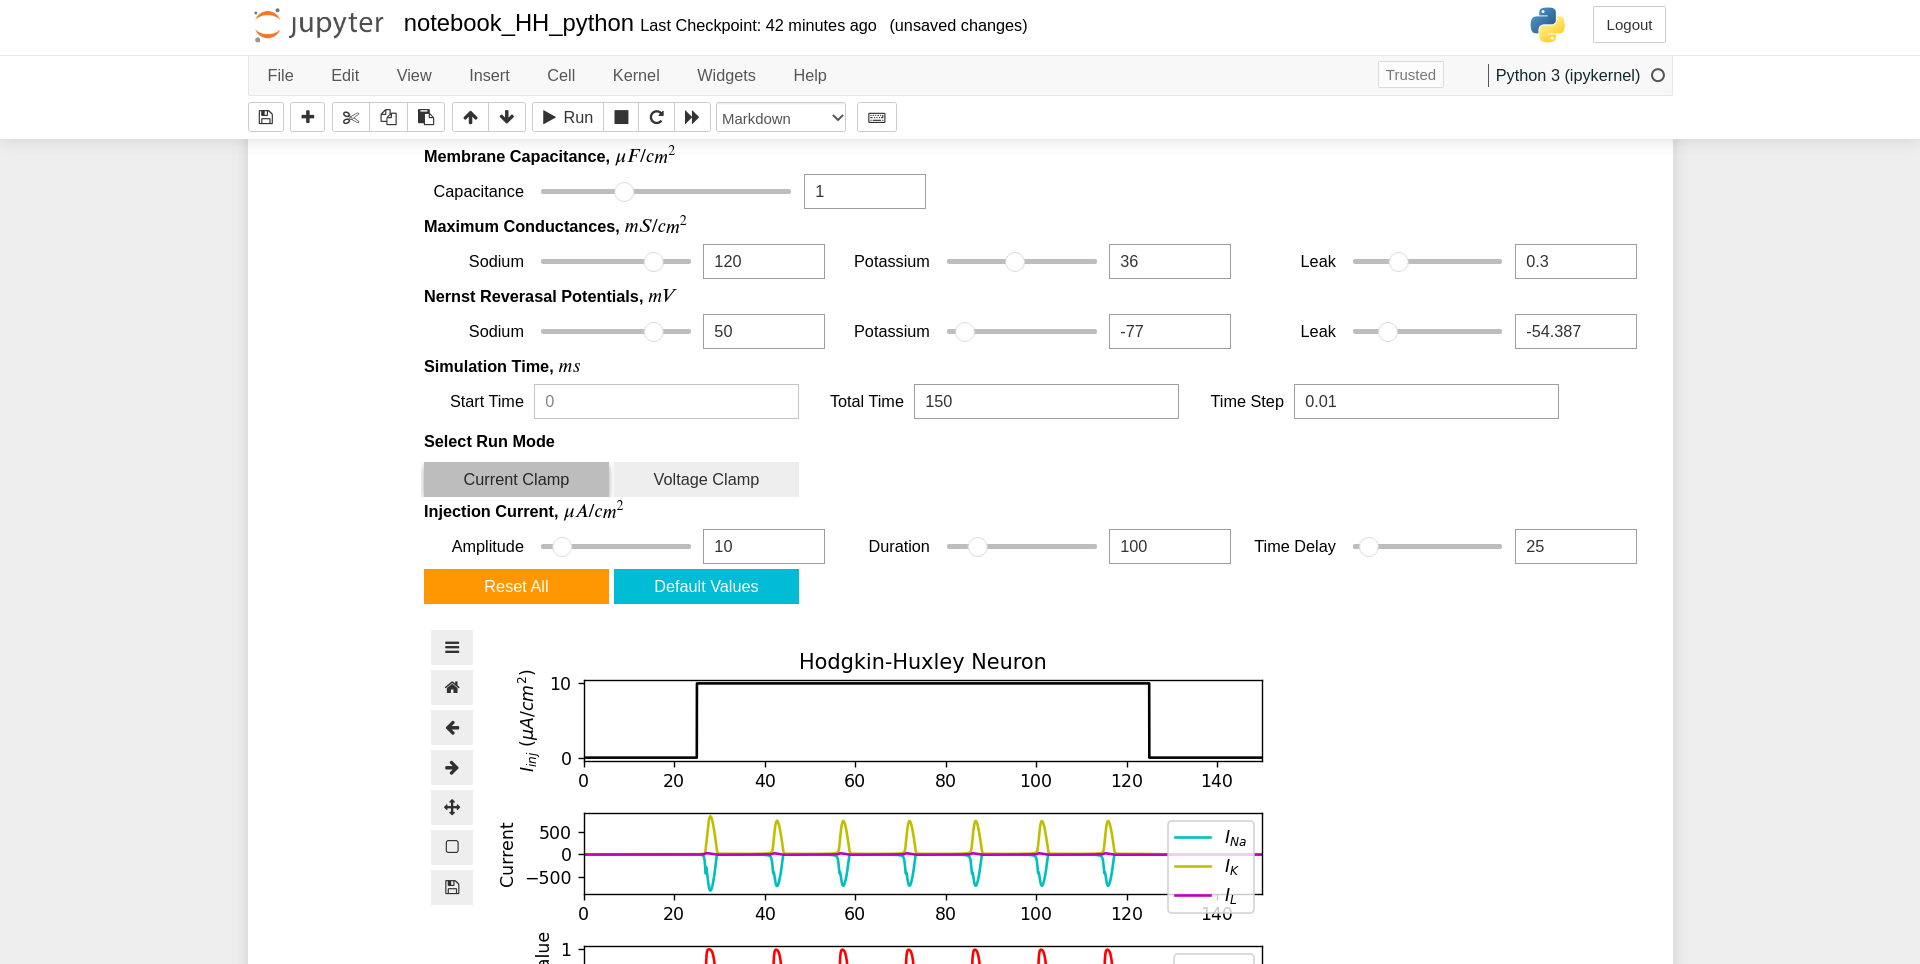
\includegraphics[width=\textwidth]{99_images/20220922-rahul-hh-1}
    \caption{Pure python tutorial converted to use Jupyter Widgets}%
    \label{fig:99_images-20220922-rahul-1}
  \end{figure}
\end{frame}
\begin{frame}[c]
  \frametitle{GSoC:\ Rahul:\ example II}
  \begin{figure}[h]
    \centering
    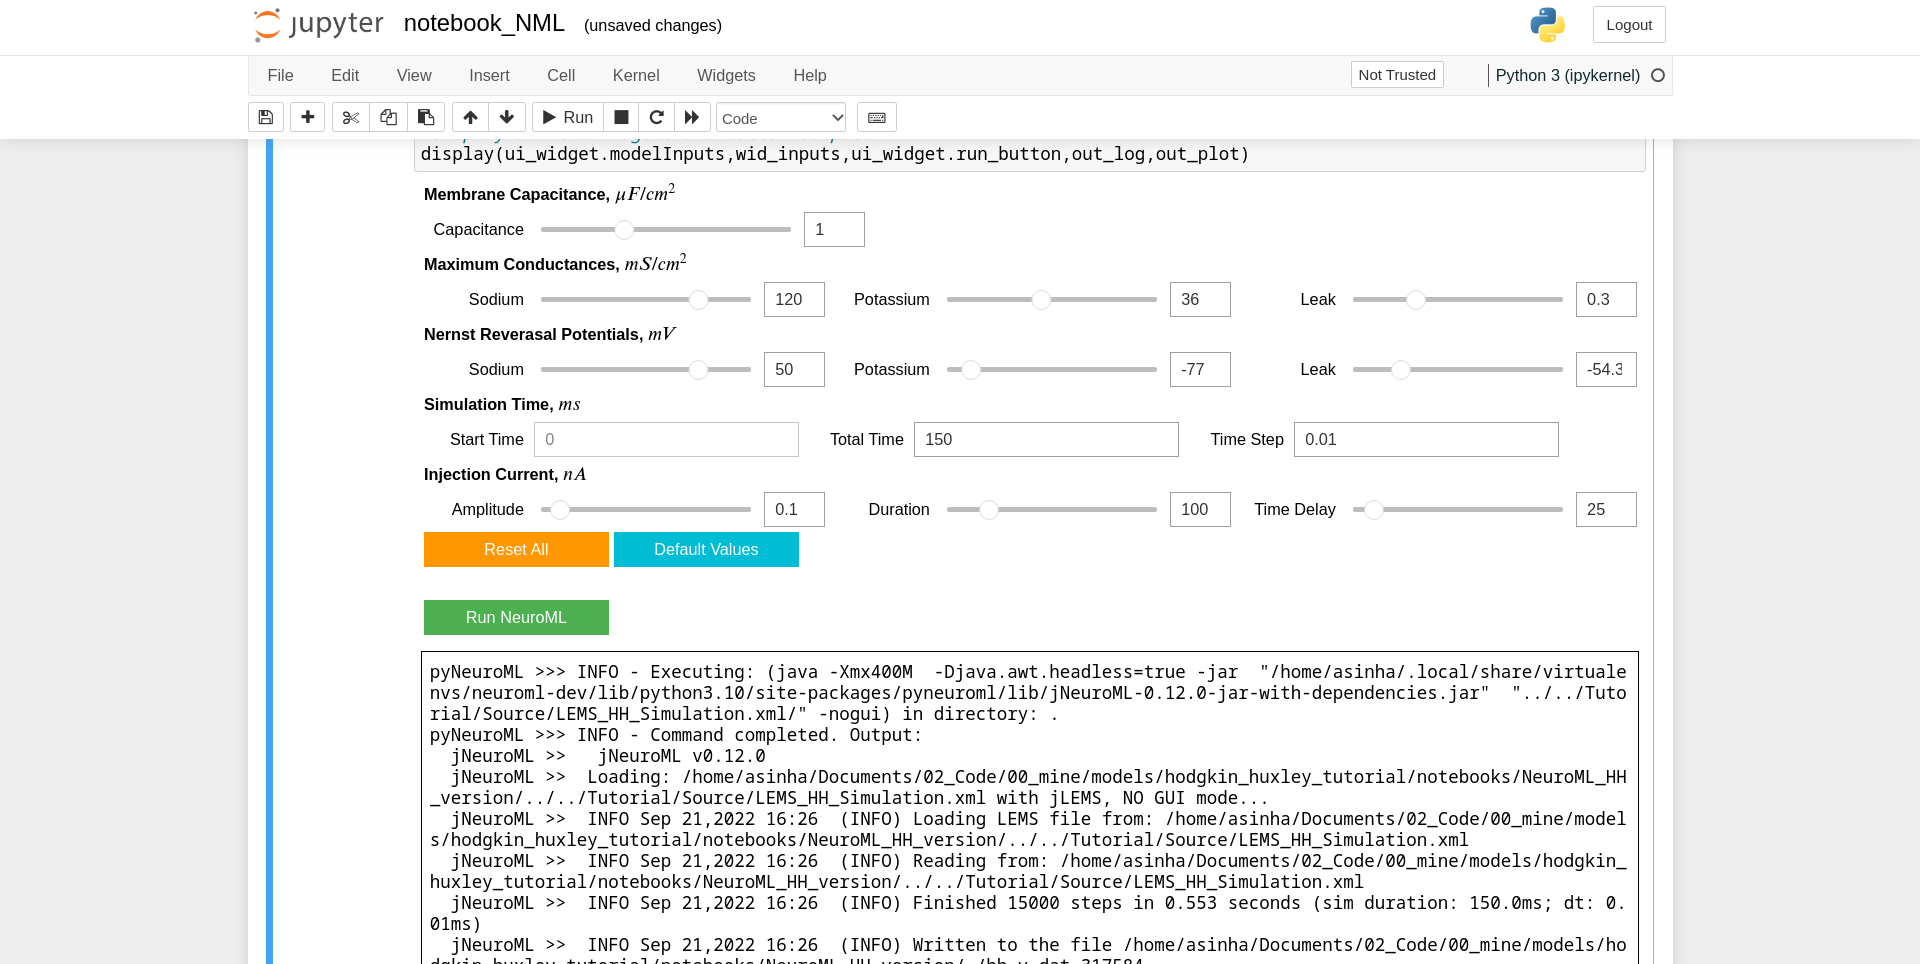
\includegraphics[width=\textwidth]{99_images/20220922-rahul-hh-2}
    \caption{NeuroML tutorial converted to use Jupyter Widgets}%
    \label{fig:99_images-20220922-rahul-2}
  \end{figure}
\end{frame}
\section{Paper and general updates}
\begin{frame}[c]
  \frametitle{Paper:\ NeuroML is the best thing since sliced bread}
  \begin{center}
    Convince readers (research community) to use NeuroML for their modelling work\textsuperscript{*}.\\\vspace{2cm}
    \pause{}
    \begin{itemize}
      \item \textsuperscript{*}instead/ahead of other tools
        \pause{}
      \item \textsuperscript{*}on a daily basis
        \begin{itemize}
          \item not as an afterthought for standardisation---once the paper has been published no one has time to re-write model (or re-process data!) to standardise
            \pause{}
            \begin{itemize}
              \item the carrot, \enquote{standardisation is good for science}, isn't enough in a mostly resource limited academic/research system
              \item requires stick:\ \enquote{for this grant, you must \ldots}; \enquote{for this journal, you must \ldots}
            \end{itemize}
        \end{itemize}
    \end{itemize}
  \end{center}
\end{frame}
\begin{frame}[c]
  \frametitle{You should use NeuroML because}
  \begin{figure}[h]
    \centering
    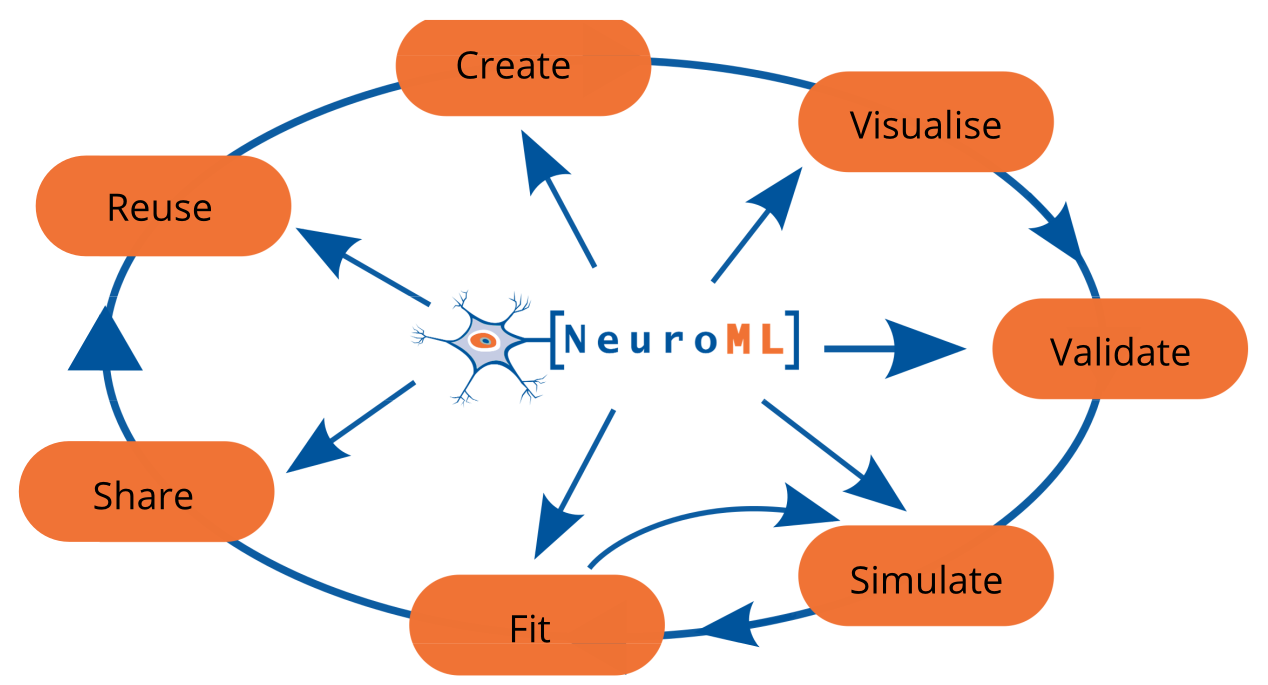
\includegraphics[width=0.8\textwidth]{99_images/neuroml-ecosystem}
    \caption{NeuroML overview figure from paper}%
    \label{fig:99_images-neuroml-ecosystem}
  \end{figure}
  \pause{}
  \begin{center}
    These claims are all true, and have been for quite a while.
  \end{center}
\end{frame}
\begin{frame}[t]
  \frametitle{So many advantages: why isn't everyone using it?}
  \pause{}
  Irrespective of all its features, NeuroML \alert{needs to be easier to use than other tools}.\\
  \pause{}%
  \begin{itemize}
    \item information on NeuroML needs to be easy to find:
      \begin{itemize}
        \item website
          \begin{itemize}
            \item point of entry for completely new users: first impression
            \item replaced with modern looking static page that redirects to individual pages in docs
            \item all information migrated to docs
          \end{itemize}
          \pause{}
        \item docs
          \begin{itemize}
            \item re-organised, modernised
            \item include tutorials, interactive tutorials via Jupyter note books, how-tos
            \item complete searchable schema docs
            \item still not yet fully complete
          \end{itemize}
      \end{itemize}
  \end{itemize}
\end{frame}
\begin{frame}[t]
  \frametitle{So many advantages: why isn't everyone using it?}
  Irrespective of all its features, NeuroML \alert{needs to be easier to use than other tools}.\\
  \begin{itemize}
    \item usability: so much can be done, but can it be done \alert{easily}?
      \begin{itemize}
        \item has not been clearly easier to use than other tools
        \item Python API exists, but we haven't taken advantage of it enough to \alert{make life easier for users} yet
      \end{itemize}
  \end{itemize}
\end{frame}
\begin{frame}[t]
  \frametitle{Example: create: single neuron Izhikevich network (from docs)}
  \inputminted[fontsize=\tiny,firstnumber=1,firstline=21,lastline=47,linenos]{python}{./extras/izhikevich-single-neuron.py}
\end{frame}
\begin{frame}[t,fragile]
  \frametitle{Inspect/visualise network}
  \begin{figure}[h]
    \centering
    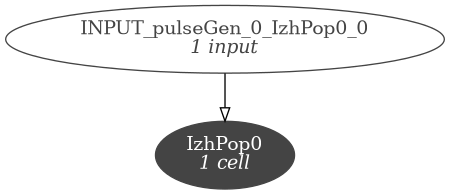
\includegraphics[width=0.25\textwidth]{99_images/IzNet.gv}
    \caption{Generated network graph}%
    \label{fig:99_images-IzNet-gv}
  \end{figure}
 \begin{minted}[breaklines=true,fontsize=\tiny]{pycon}
>>> nml_doc.summary()
*******************************************************
* NeuroMLDocument: IzhSingleNeuron
*
*  Izhikevich2007Cell: ['izh2007RS0']
*  PulseGenerator: ['pulseGen_0']
*
*  Network: IzNet
*
*   1 cells in 1 populations 
*     Population: IzhPop0 with 1 components of type izh2007RS0
*
*   0 connections in 0 projections 
*
*   0 inputs in 0 input lists 
*
*   1 explicit inputs (outside of input lists)
*     Explicit Input of type pulseGen_0 to IzhPop0(cell 0), destination: unspecified
*
*******************************************************
 \end{minted}
\end{frame}
\begin{frame}[t]
  \frametitle{Strengths}
  \begin{itemize}
      \item extremely \alert{declarative}
        \begin{itemize}
          \item components (Izhikevich2007Cell, Network, Population, PulseGenerator, ExplicitInput) clearly visible
          \item components and dynamics fully, formally documented in schema docs
          \item component parameters clearly visible
          \item units/dimensions explicitly mentioned
        \end{itemize}
  \end{itemize}
\end{frame}
\begin{frame}[t]
  \frametitle{Strengths}
  \begin{figure}[h]
    \centering
    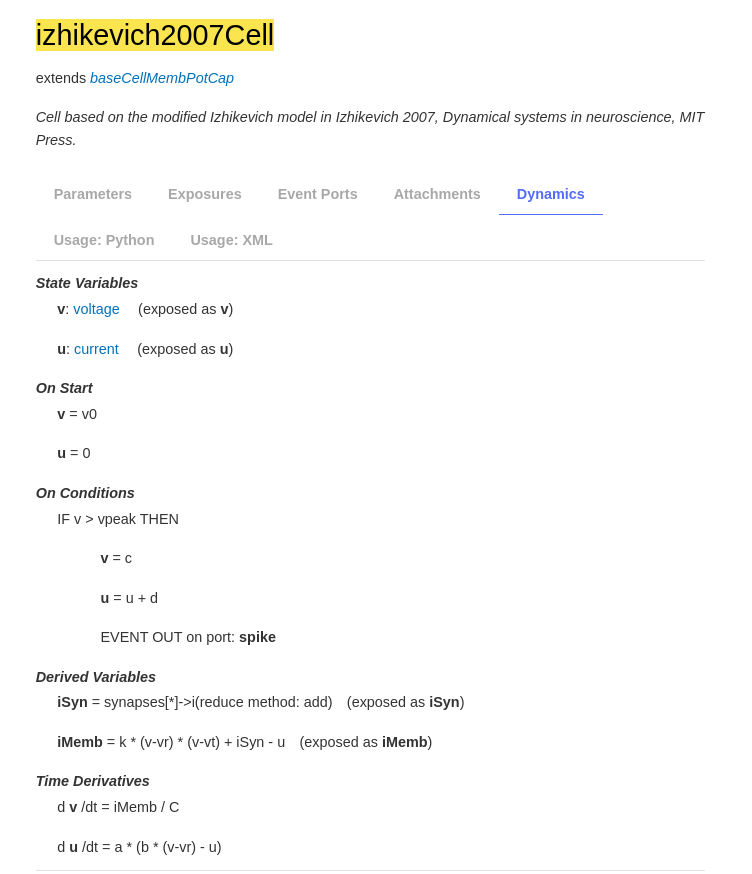
\includegraphics[width=0.55\textwidth]{99_images/izhikevich-schema-docs}
    \caption{Schema docs on Izhikevich2007Cell}%
    \label{fig:99_images-izhikevich-schema-docs}
  \end{figure}
\end{frame}
\begin{frame}[t]
  \frametitle{Strengths}
  \begin{itemize}
      \item \alert{validation} without simulation (no simulator has this)
        \begin{itemize}
          \item Level 1 validation: units/dimensions, structure of model checked against schema
          \item Level 2 validation: extra \enquote{logical} checks
        \end{itemize}
        \pause{}
      \item easy \alert{simulation} with different simulators
      \item easy \alert{visualisation} and inspection of model: network structure, connectivity matrices, LEMS simulation graph, morphology figures, model summary
  \end{itemize}
\end{frame}
\begin{frame}[t]
  \frametitle{Weaknesses}
  \begin{itemize}
    \item information on components: must switch back and forth between docs and code
      \begin{itemize}
        \item Not too bad: required for most simulators/programming languages
      \end{itemize}
      \pause{}
    \item unclear how components fit together
      \begin{itemize}
        \item how do I know that Network \textrightarrow{} Populations \textrightarrow{}?
      \end{itemize}
      \pause{}
    \item Too many \enquote{under the hood} bits that users are expected to know:
      \begin{itemize}
        \item \mintinline[fontsize=\small]{python}{nml_doc.izhikevich2007_cells.append(izh0)}
        \item how do users know this?
          \begin{itemize}
            \item read the schema docs?
            \item read the \href{https://libneuroml.readthedocs.io/en/development/userdocs/coreclasses.html?highlight=neuromldocument\#neuromldocument}{NeuroML Python API documentation?} 
            \item read the \href{https://github.com/NeuralEnsemble/libNeuroML/blob/master/neuroml/nml/nml.py}{NeuroML Python API source?} (currently 64,000 lines of code)
          \end{itemize}
      \end{itemize}
  \end{itemize}
\end{frame}
\begin{frame}[t]
  \frametitle{Weaknesses}
  \begin{itemize}
    \item validation upon model completion
      \begin{itemize}
        \item using \texttt{jnml}, so requires Java
        \item better than errors on run, but still quite late
      \end{itemize}
      \pause{}
    \item NeuroML generated NEURON code is less performant than native NEURON code
      \begin{itemize}
        \item because hand-written mod files can be optimised, while we rely on a template to generate them
        \item TODO:\ optimisation of template
      \end{itemize}
  \end{itemize}
\end{frame}
\begin{frame}[t]
  \frametitle{Example: create: single neuron Izhikevich network (devel)}
  \inputminted[fontsize=\tiny,firstnumber=1,firstline=17,lastline=42,linenos]{python}{./extras/izhikevich-single-neuron-dev.py}
\end{frame}
\begin{frame}[t,fragile]
  \frametitle{The component factory}
  \begin{itemize}
    \item single factory function to create new components
    \item runs extra checks
      \begin{itemize}
        \item are all arguments (parameters) correct?
        \item is the component valid (level 1 validation for each component at build-time)?
      \end{itemize}
  \end{itemize}
 \begin{minted}[breaklines=true,fontsize=\tiny]{pycon}
>>> izh0 = component_factory("Izhikevich2007Cell")
ValueError: Validation failed:
- Izhikevich2007Cell (None): Required value v0 is missing
- Izhikevich2007Cell (None): Required value k is missing
- Izhikevich2007Cell (None): Required value vr is missing
- Izhikevich2007Cell (None): Required value vt is missing
- Izhikevich2007Cell (None): Required value vpeak is missing
- Izhikevich2007Cell (None): Required value a is missing
- Izhikevich2007Cell (None): Required value b is missing
- Izhikevich2007Cell (None): Required value c is missing
- Izhikevich2007Cell (None): Required value d is missing
- Izhikevich2007Cell (None): Required value C is missing
- Izhikevich2007Cell (None): Required value id is missing
 \end{minted}
\end{frame}
\begin{frame}[t,fragile]
  \frametitle{The component factory}
 \begin{minted}[breaklines=true,fontsize=\tiny]{pycon}
>>> izh0 = component_factory(
      "Izhikevich2007Cell",
      id="izh2007RS0", v0="-60mV", C="100pF", k="0.7nS_per_mV", vr="-60mV",
      vt="-40ms", vpeak="35mV", a="0.03per_ms", b="-2nS", c="-50.0mV", d="100pA")

ValueError: Validation failed:
 - Izhikevich2007Cell (izh2007RS0): Value "-40mS" does not match xsd pattern restrictions: [['^(-?([0-9]*(\\.[0-9]+)?)([eE]-?[0-9]+)?[\\s]*(V|mV))$']]]
 \end{minted}
\end{frame}
\begin{frame}[t,fragile]
  \frametitle{New add method}
  \begin{itemize}
    \item uses component factory to create a new component and run checks
    \item smart enough to know where the new element needs to go in the parent
  \end{itemize}
  \begin{center}
    \inputminted[fontsize=\tiny,firstnumber=1,firstline=23,lastline=26,linenos]{python}{./extras/izhikevich-single-neuron.py}
    vs
    \inputminted[fontsize=\tiny,firstnumber=1,firstline=20,lastline=23,linenos]{python}{./extras/izhikevich-single-neuron-dev.py}
  \end{center}
\end{frame}
\begin{frame}[t,fragile]
  \frametitle{Inspect each component individually}
  \begin{minted}[breaklines=true,fontsize=\tiny]{pycon}
izh0.info(show_contents=True)
Izhikevich2007Cell -- Cell based on the modified Izhikevich model in Izhikevich 2007, Dynamical systems in neuroscience, MIT Press
Please see the NeuroML standard schema documentation at https://docs.neuroml.org/Userdocs/NeuroMLv2.html for more information.

Valid members for Izhikevich2007Cell are:
* b (class: Nml2Quantity_conductance, Required)
        * Contents ('ids'/<objects>): -2nS

* C (class: Nml2Quantity_capacitance, Required)
        * Contents ('ids'/<objects>): 100pF

* c (class: Nml2Quantity_voltage, Required)
        * Contents ('ids'/<objects>): -50.0mV

* d (class: Nml2Quantity_current, Required)
        * Contents ('ids'/<objects>): 100pA

* neuro_lex_id (class: NeuroLexId, Optional)
* metaid (class: MetaId, Optional)
* v0 (class: Nml2Quantity_voltage, Required)
        * Contents ('ids'/<objects>): -60mV

* id (class: NmlId, Required)
        * Contents ('ids'/<objects>): izh2007RS0
  ...
  \end{minted}
\end{frame}
\begin{frame}[t,fragile]
  \frametitle{Component Type info without creating a new component: ctinfo}
  \begin{minted}[breaklines=true,fontsize=\tiny]{pycon}
>>> ctinfo("ExpOneSynapse")
ExpOneSynapse -- Ohmic synapse model whose conductance rises instantaneously by ( **gbase**  * **weight**  ) on receiving an event, and which decays exponentially to zero with time course **tauDecay**

Please see the NeuroML standard schema documentation at https://docs.neuroml.org/Userdocs/NeuroMLv2.html for more information.

Valid members for ExpOneSynapse are:
* neuro_lex_id (class: NeuroLexId, Optional)
* gbase (class: Nml2Quantity_conductance, Required)
* metaid (class: MetaId, Optional)
* erev (class: Nml2Quantity_voltage, Required)
* notes (class: xs:string, Optional)
* id (class: NmlId, Required)
* properties (class: Property, Optional)
* annotation (class: Annotation, Optional)
* tau_decay (class: Nml2Quantity_time, Required)

  \end{minted}
\end{frame}
\begin{frame}[t,fragile]
  \frametitle{Where does this component type fit?}
  \begin{minted}[breaklines=true,fontsize=\tiny]{pycon}
>>> ctparentinfo("HHRate")
Please see the NeuroML standard schema documentation at https://docs.neuroml.org/Userdocs/NeuroMLv2.html for more information.

Valid parents for HHRate are:
* GateHHRates
        * forward_rate (class: HHRate, Required)
        * reverse_rate (class: HHRate, Required)
* GateHHRatesInf
        * forward_rate (class: HHRate, Required)
        * reverse_rate (class: HHRate, Required)
* GateHHRatesTau
        * forward_rate (class: HHRate, Required)
        * reverse_rate (class: HHRate, Required)
* GateHHRatesTauInf
        * forward_rate (class: HHRate, Required)
        * reverse_rate (class: HHRate, Required)
* GateHHUndetermined
        * forward_rate (class: HHRate, Optional)
        * reverse_rate (class: HHRate, Optional)
  \end{minted}
\end{frame}
\begin{frame}[t,fragile]
  \frametitle{Additions to make multi-compartment cell building easier}
  \begin{itemize}
    \item \mintinline{python}{set_init_memb_potential()} instead of \mintinline[fontsize=\tiny]{python}{cell.biophysical_properties.membrane_properties.init_memb_potential}
    \item \mintinline{python}{add_channel_density()}\ldots
    \item \mintinline{python}{add_segment}, \mintinline{python}{add_unbranched_segment_list}\ldots
      \begin{itemize}
        \item also takes care of \href{https://scicrunch.org/scicrunch/interlex/dashboard}{NeuroLex} (now InterLex) Ids, used by NEURON to create \enquote{sections}.
        \item another hidden feature of NeuroML
      \end{itemize}
  \end{itemize}
\end{frame}
\begin{frame}[t]
  \frametitle{On-going/future work: not all to be done before paper}
  \begin{itemize}
    \item more utils for other common, repeated tasks (model factory/templates?)
    \item update docs, add more tutorials/recipes
      \pause{}
    \item GUI model building
      \begin{itemize}
        \item Jupyter widgets based model inspection/modification/creation
        \item NeuroMLLite GUI (NeuroML v3?)
          \begin{itemize}
            \item Will absorb all neuroConstruct functionality
          \end{itemize}
      \end{itemize}
      \pause{}
    \item Complete NetPyNE UI interactions with NeuroML
      \begin{itemize}
        \item import works, but cannot modify model
        \item export needs to be implemented
      \end{itemize}
      \pause{}
    \item Migrate all code to Python (so no more Java required)
      \begin{itemize}
        \item long term, multi-year project, requires another grant
      \end{itemize}
  \end{itemize}
\end{frame}
\end{document}
